\vspace{-0.1in}
\section{Introduction}
\vspace{-0.05in}
\label{sec:intro}
Existing datacenters are based on a server-centric architecture, in which a small amount of the various resources needed for computing tasks (CPU, memory, storage) are tightly integrated within a single server. While server-centric architectures have been the mainstay for decades, recent efforts suggest a paradigm shift towards a {\em disaggregated} datacenter (\dis) that is architected as a pool of decoupled resources. In \dis, each resource type is built as a standalone resource `blade' and all blades are interconnected via a unified network fabric as shown in Figure~\ref{fig:dc}. In such a datacenter, the aggregation of resources needed by a job is then logical (allocated by a software scheduler) rather than physical (dictated by hardware).

Multiple small-scale prototypes of disaggregated hardware exist already --- Intel RSA~\cite{rsa}, HP ``the machine''~\cite{hptm}, Facebook's disaggregated rack~\cite{fdr}, and SeaMicro~\cite{seamicro}, as well as research prototypes like Firebox~\cite{firebox}, soNUMA~\cite{sonuma}, and memory blades~\cite{ddcHwDesign1}.

\begin{figure*}[!t]
\centering 
\subfigure[Current datacenter] {
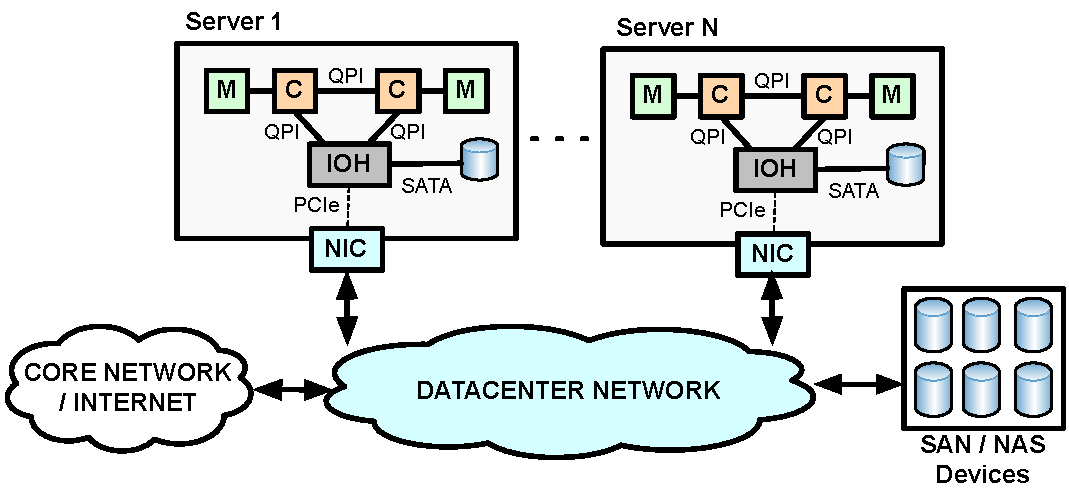
\includegraphics[width=3.05in]{img/DC_before_4.pdf}
\label{fig:dc_before}
}
\hfill
\subfigure[Disaggregated datacenter] {
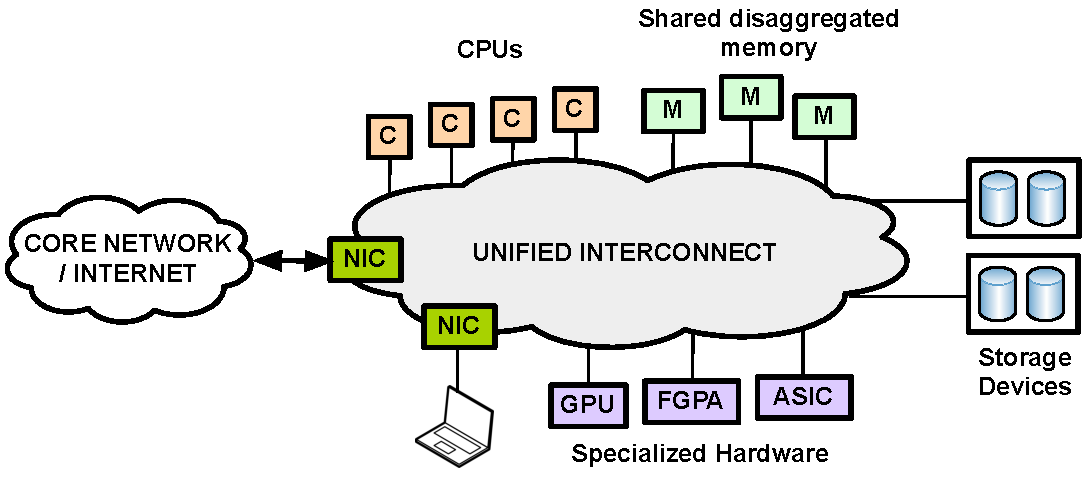
\includegraphics[width=3.05in]{img/DC_after_2.pdf}
\label{fig:dc_after}
}
\tightcaption{Architectural differences between server-centric and resource-centric datacenters}
\label{fig:dc}
\end{figure*}


Resource disaggregation stands to benefit both hardware developers and datacenter operators. %is beneficial along several dimensions. 
For hardware developers, disaggregation makes hardware more modular and hence 
easier to build and evolve. 
For example, an ongoing challenge for hardware architects is that technologies for CPUs, memory, storage, etc. have very different cost, performance, and power scaling trends and this constrains their integration; e.g., architects have warned of an impending `memory capacity wall' making the co-location of compute and memory in a single server unsustainable~\cite{ddcHwDesign1}. 
Similarly, as new needs or technologies arise~\cite{memristors,nvram,reg-ex-hardware,gpus}, having standalone per-resource blades avoids the burdensome process of redoing the process of integration and motherboard design.
%, and server factor form planning. 
Disaggregation offers similar benefits to operators, as it enables finer-grained control over how they  provision, upgrade, and schedule individual resources.
%Finally, resource disaggregation allows overcoming the technology barriers (imbalance between memory and CPU capacity, power dissipation issues, etc), potentially enabling new technological advances. 

While disaggregation offers many benefits, it introduces new challenges for the underlying network fabric. Today's servers offer high bandwidth and low latency communication between the resources within the server (see Table~\ref{tab:tech}). However, with disaggregation, some of the inter-resource communication that used to be contained within a server must now traverse the external network fabric. This not only increases the load on the network but makes low latency communication on the fabric critical. The network will thus be a key enabling or limiting factor in realizing resource disaggregation. 
Despite the central role that the network plays in \dis, there has been little systematic evaluation of the requirements or feasibility of scaling networks for disaggregation. Instead, existing prototypes of disaggregated platforms have been small scale and/or proprietary~\cite{rsa, hptm, fdr, seamicro}. 

This paper takes a first step towards understanding what network support is required for resource disaggregation. Rather than approach the question from a clean-slate, we adopt a workload-driven approach: we take five diverse workloads commonly found in today's datacenters -- batch processing jobs in Hadoop and Spark, point queries with memcached~\cite{memcached} and ElasticSearch~\cite{elastic}, streaming jobs in Storm~\cite{storm} -- and address three questions in the context of these workloads: 
%through a combination of emulations and simulation: 

\cut{
\vspace{-0.5em}
\begin{itemize}[leftmargin=*]
	\itemsep0em
	\item What network latency and bandwidth are required to avoid degrading application-level performance relative to server-centric architectures? 
	\item How (and why) does disaggregation change network traffic characteristics such as flow size distributions, communication patterns, traffic volumes, burstiness, and so forth?
    \item Can existing transport protocols meet the above requirements? 
\end{itemize}
}

\noindent {\bf (1) Network performance requirements:} What network latency and bandwidth are required to avoid degrading application-level performance relative to server-centric architectures? 

\noindent {\bf (2) Traffic workloads:} How (and why) does disaggregation change network traffic characteristics such as flow size distributions, communication patterns, traffic volumes, burstiness, and so forth?

\noindent {\bf (3) L3 and L4 protocol support:} Can existing (deployed or proposed) network designs meet the above requirements?


\cut{ 
%SR: need to find a place to discuss this (but not here)
To date, there is no consensus on the granularity at which resource disaggregation will happen --- at the rack-scale, pod-scale, or an extreme of datacenter scale. Moreover, as briefly discussed above, resource disaggregation enables flexibility in choice of provisioning and sharing of resources adding to the degrees of freedom in design of \dis architecture. Given that our focus is on understanding the network support for \dis (rather than proposing a \dis architecture), we consider the new degrees of freedom --- scale of disaggregation, CPU-memory disaggregation, data placement and access, etc. --- as design parameters that may impact our study. 
} 

\vspace{0.5em}
\noindent Our key findings are as follows:
\vspace{-0.5em}
\begin{itemize}[leftmargin=*]
	\itemsep0em
		\item To maintain application performance comparable to current datacenters, a disaggregated datacenter must provide at least $40$Gbps bandwidth to end-points and an end-to-end latency of no more than $5\mu$s.
		\item Traffic workloads in a disaggregated datacenter will differ significantly from existing workloads. Specifically, we observe: (a) \sr{quantify? e.g. X-times?} more homogeneous spatial and temporal distribution of traffic; (b) a \sr{X} lower skew in flow size distributions with a long flows, and (c) a \sr{X} increase in overall traffic volume, with a \sr{Z} more uniform distribution of bytes between short {\em vs.} long flows.
		\item We evaluate four transport protocols -- TCP, pFabric~\cite{pfabric}, pHost~\cite{phost}, and  FastPass~\cite{fastpass} -- for their ability to provide low end-to-end latencies with \dis workloads and find that, while pFabric and pHost can meet \dis requirements, FastPass and TCP fail to do so. 
		\item \sr{TODO: let's discuss} scale: surprisingly, not an important factor; primary factors are the app's memory access pattern and bandwidth.
		\end{itemize} 
	
	
%	We discuss how the above findings inform future research in \S\ref{sec:workloads}.
Taken together we view our results as encouraging in that they suggest that commodity networking technology and existing design practices -- e.g., Ethernet links, droptail and priority switching, end-to-end reliability, etc. -- are within reach of meeting the needs of \dis. This finding is in contrast to early prototypes of disaggregated platforms (from the hardware community) that build new network fabrics often resembling intra-server interconnects; e.g., with Torus  topologies~\cite{sea-micro}, new link types~\cite{intel-si-photonics}, per-hop reliability, etc. \sr{check!!} Thus we hope our results lead to a broader exploration of the network requirements for \dis.
	
	\cut{
	%SR: cut because intro was too long. 
	For example,
	while $40$Gbps (or even $100$Gbps) is feasible today, achieving end-to-end latencies of $5\mu$ remains challenging. 
	Similarly, network designs have often been guided by measurement studies that provided models of traffic workloads~\cite{srikanth,theo}; e.g., the prevalence of `elephant' flows led to new proposals for routing~\cite{vahdat-something}, load-balancing~\cite{flowlets}, new hybrid electrical-optical or electrical-wireless~\cite{dga-something, vyas-something, msr-something} network designs, and so forth. 
	With a radically different traffic workload (e.g., the disappearance of elephant flows), many common design assumptions should be re-examined.
	}
        %\item Short memory-bound flows dominating the \dis traffic, combined with a more homogeneous spatial and temporal traffic distribution present favorable characteristics for existing transport protocols~\cite{pfabric} to meet \dis requirements. %However, depending on the design parameters, existing protocols may be subjected to new challenges namely, robustness across workloads and application-level policies on flow prioritization (\S\ref{sec:existing}).

\noindent
We note three limitations of our work. First, our results are based on five specific workloads; we leave to future work an  evaluation of whether our results generalize to other applications.%, including applications (re)written to exploit disaggregation. 
Second, we focus primarily on questions of \emph{network} design for disaggregation, ignoring many systems-related questions (e.g., software stack or scheduler designs). However, the latter may well turn out to be the more critical bottleneck for disaggregation. In this sense, one might view our study as exploring whether the network can `get out of the way' (as is often advocated~\cite{greenberg-sigcomm15, vahdat-something}) even under disaggregation. Finally, our work looks ahead to an overall system  that does not yet exist and hence we must make assumptions on certain fronts (e.g., data layout, rack organization (\S\ref{ssec:system}). We make what we believe are sensible choices and state these choices explicitly.
%: not for layout or rack org?, and in many cases, explore how these choices impact our results. 
Nonetheless, our results are dependent on these choices and more experience is needed to confirm their validity.

\cut{
\noindent
\sr{Add a list of caveats/disclaimers as follows\ldots}
\begin{itemize} 
\item our results are based on the workloads we study; not comprehensive
\item we focus on net design, ignore many systems questions; may still well turn out that the latter matters more; in this sense one might view our study as seeing whether the network can `get out of the way’ \cite{};
\item because our study is forward looking, many aspects of the overall context we’re considering don’t exist yet so we must make assumptions - e.g., data layout, how resources blades are organized, etc.  We 
\end{itemize} 
}